% !TEX root=SysSpec_ClockPendulumAnalyzer
\subsection{Umsetzung des GPIO Zugriff}
Der Zugriff auf die GPIO Pins des Raspberry wurde mit einer simplen Klasse umgesetzt. Diese Klasse ist verantwortlich für das Exportieren und Unexportieren der Pins. Dies geschieht bei der Initialisierung der Klasse beziehungsweise beim Dekonstruktor. Dabei wird das Prinzip der Resourcenbelegung ist Initialisierung (kurz RAII) nicht verletzt.\\
\\
Die Aufgaben des Benutzers sind nur Richtung setzen und dann Lesen bzw. Schreiben der Pins. Die Richtung (Output / Input) kann zur Laufzeit geändert werden.

\subsubsection{Pinbelegung}
Die Pinbelegung auf dem Raspberry Pi 3 sieht wie folgt aus.
\begin{figure}[H]
    \centering
    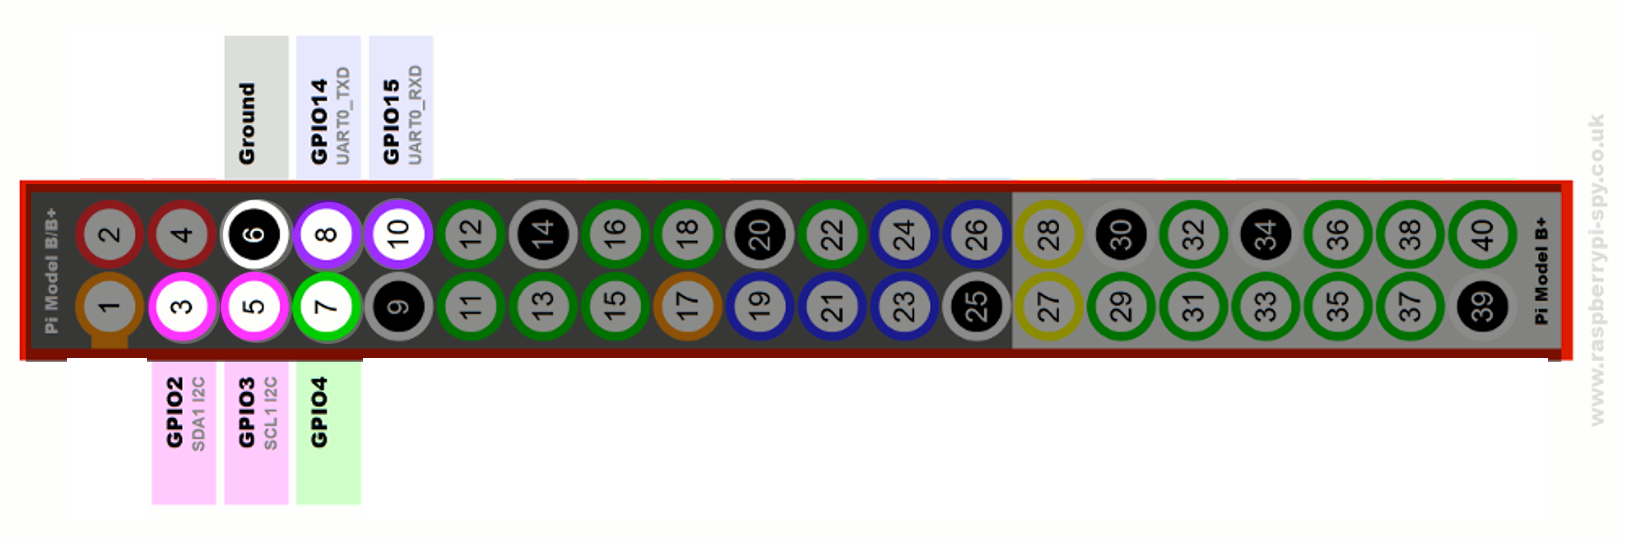
\includegraphics[width=\textwidth]{pinbelegung}
    \caption{Pinbelegung des Raspberry (Originalbild von www.raspberrypi-spy.co.uk)}
\end{figure}

\noindent Pin 6,8,10,3 und 5 werden nicht durch die GPIO Klasse angesteuert. Diese sind für die UART bzw. $I^2C$ Kommunikation reserviert.\\\\
Pin 7 dient als Interrupt-Pin für den Hardware Counter. Dieser wird bei Programmstart als High Output Pin gesetzt um damit den Counter zurückzusetzen. Damit wird erreicht, dass das System auf unterschiedliche Aufstartzeiten reagieren kann und die ganze Messung gleichzeitig starten kann. Der Counter-Reset wird nur bei Programmstart ausgeführt und danach nicht mehr.

\subsubsection{I2C Implementierung}
Der I2C Anschluss läuft über Pin 3 (SDA\footnote{Data Signal}) und 5 (SCL\footnote{Clock Signal}).\\
Für den I2C wurde ebenfalls eine abstrahierende Klasse entwickelt. Diese verwendet die bereits vom Linux bereitgestellten Funktionalitäten zum Lesen und Schreiben von I2C-Geräten.\\
\\
Im Kontext des Clock Pendulum Analyzers wird die I2C Kommunikation zwischen RTC, Counter und Raspberry verwendet. Dabei ist das Raspberry der Master und fordert die anderen zwei Teilnehmer nach ihren Daten.\\
Der Counter hat dabei die Adresse %TODO Counter Adresse für i2c
und die RTC wird über Adresse %TODO RTC Adresse für i2c
angesprochen.

\subsubsection{UART Implementierung}\label{sec:uart}
Für das Lesen des GPS Signals wird eine UART Kommunikation benötigt. Diese wird ebenfalls wie die oberen Klassen abstrahiert und bietet somit einfache Lese- und Schreibemöglichkeit.\\
\\
Die UART Verbindung läuft über die Pins 8 (Tx, Transmitter) und 10 (Rx, Receiver).\\
Als Komponente des UARTs wird die Adafruit\_GPS Bibliothek\footnote{Adafruit GPS Repository \cite{adafruit}} verwendet. Diese bietet bereits eine vereinfachte  Kommunikation mit dem GPS. Mit Wrapperfunktionen wird der Setup und das Beenden nochmals abstrahiert.\\
Für die Kommunikation mit dem GPS wird eine Standardgeschwindigkeit (Baudrate) von 9600 gewählt. Vom GPS benötigt das Raspberry nur die Zeit und daher werden nur diese abgefragt.
